\chapter{Literatuurstudie}
\label{ch:literatuurstudie}

% Tip: Begin elk hoofdstuk met een paragraaf inleiding die beschrijft hoe
% dit hoofdstuk past binnen het geheel van de bachelorproef. Geef in het
% bijzonder aan wat de link is met het vorige en volgende hoofdstuk.

Deze literatuurstudie zal samen met de lijst van termen uit hoofdstuk \ref{ch:termen} de nodige achtergrondinformatie bieden om de volgende delen van de paper te begrijpen. Er zal verwezen worden naar meerdere papers van andere instellingen zodat u zich verder kan inlezen waar gewenst.

% Pas na deze inleidende paragraaf komt de eerste sectiehoofding.


%Dit hoofdstuk bevat je literatuurstudie. De inhoud gaat verder op de inleiding, maar zal het onderwerp van de bachelorproef *diepgaand* uitspitten. De bedoeling is dat de lezer na lezing van dit hoofdstuk helemaal op de hoogte is van de huidige stand van zaken (state-of-the-art) in het onderzoeksdomein. Iemand die niet vertrouwd is met het onderwerp, weet nu voldoende om de rest van het verhaal te kunnen volgen, zonder dat die er nog andere informatie moet over opzoeken \autocite{Pollefliet2011}.

%Je verwijst bij elke bewering die je doet, vakterm die je introduceert, enz. naar je bronnen. In \LaTeX{} kan dat met het commando \texttt{$\backslash${textcite\{\}}} of \texttt{$\backslash${autocite\{\}}}. Als argument van het commando geef je de ``sleutel'' van een ``record'' in een bibliografische databank in het Bib\LaTeX{}-formaat (een tekstbestand). Als je expliciet naar de auteur verwijst in de zin, gebruik je \texttt{$\backslash${}textcite\{\}}.
%Soms wil je de auteur niet expliciet vernoemen, dan gebruik je \texttt{$\backslash${}autocite\{\}}. In de volgende paragraaf een voorbeeld van elk.


%\textcite{Knuth1998} schreef een van de standaardwerken over sorteer- en zoekcompressie-algoritmen. Experten zijn het erover eens dat cloud computing een interessante opportuniteit vormen, zowel voor gebruikers als voor dienstverleners op vlak van informatietechnologie~\autocite{Creeger2009}.

\section{Bestandsgrootte en dataopslag}
\label{sec:bestandsgrootte-dataopslag}
Zoals in de definitie van \gls{datacompressie} besproken is, bestaat \gls{datacompressie} uit het digitaal opslaan van een bestand met zo weinig mogelijk \glspl{bit}.

\Gls{bit} staat kort voor binary digit. Een bit wordt beschouwd als de kleinste data eenheid voor dataopslag. Een bit kan twee waarden aannemen, deze worden voorgesteld door 1 of 0 (binair talstelsel), maar kunnen ook geïnterpreteerd worden als aan of uit, ja of nee…

\subsection{Voorvoegsels voor het uitdrukken van bestandsgrootte}
\label{sec:bestandsgrootte-dataopslag-voorvoegsels}

Bestandsgroottes worden meestal uitgedrukt in bytes (8 bits), al dan niet met voorvoegsel dat een veelvoud voorstelt. Deze voorvoegsels en het door elkaar gebruik van de \gls{si-voorstelling-bestandsgrootte} en \gls{binaire-voorstelling-bestandsgrootte} kan voor enige verwarring zorgen. Denk hierbij aan het fenomeen dat harde schijven die geadverteerd zijn als 1TB (\gls{si-voorstelling-bestandsgrootte}) overeen komen met 931GiB (\gls{binaire-voorstelling-bestandsgrootte}) op de meeste besturingssystemen. Doorheen deze paper zal de \gls{si-voorstelling-bestandsgrootte} gebruikt worden.

\subsubsection{SI voorstelling}
\label{sec:bestandsgrootte-dataopslag-voorvoegsels-si}

De \gls{si-voorstelling-bestandsgrootte} gebruikt als basis 1000 wat overeen komt met $ 10^{3} $. SI staat voor International System of Units en beschrijft de standaardeenheden voor het meten van bepaalde data. Het wordt beschouwd als een moderne vorm op het metrisch stelsel. SI beschrijft onder IEC 60027 het gebruik van bepaalde voorvoegsels voor het uitdrukken van machten op 10. (\cite{iec60027}) Een conversietabel is hieronder raadpleegbaar. 

\FloatBarrier
\begin{table}[h]
	\begin{tabular}{|l|l|l|}
		\hline
		\textbf{Voorvoegsel} & \textbf{symbool} & \textbf{waarde} \\ \hline
		kilo & Ki & $ 10^{3} = 1000^{1} $  = 1 000 \\ \hline
		mega & Mi & $ 10^{6} = 1000^{2} $  = 1 000 000 \\ \hline
		giga & Gi & $ 10^{9} = 1000^{3} $  = 1 000 000 000 \\ \hline
	\end{tabular}
\end{table}
\FloatBarrier

\subsubsection{Binaire voorstelling}
\label{sec:bestandsgrootte-dataopslag-voorvoegsels-binair}

De \gls{binaire-voorstelling-bestandsgrootte} gebruikt als basis 1024, wat overeen komt met $ 2^{10} $. Deze voorstelling is een standaardisatie opgelegd door \gls{ieee} 1541-2002 (\cite{ieee15412002}). Een conversietabel is hieronder raadpleegbaar.

\FloatBarrier
\begin{table}[h]
	\begin{tabular}{|l|l|l|}
		\hline
		\textbf{Voorvoegsel} & \textbf{symbool} & \textbf{waarde} \\ \hline
		kibi & Ki & $ 2^{10} = 1024^{1} $  = 1 024 \\ \hline
		mebi & Mi & $ 2^{20} = 1024^{2} $ = 1048 576 \\ \hline
		gibi & Gi & $ 2^{30} = 1024^{3} $ = 1 073 741 824 \\ \hline
	\end{tabular}
\end{table}
\FloatBarrier

\subsubsection{Clustergrootte}
\label{sec:bestandsgrootte-dataopslag-clustergrootte}

Een andere belangrijke term bij dataopslag is de \gls{clustergrootte}. Data moet namelijk bijgehouden worden in één of meerdere \glspl{cluster} op een opslagmedium zodat naar deze \glspl{cluster} kan verwezen worden voor het lezen van de data. 

Aangezien alle data steeds minstens in één \gls{cluster} staat en twee verschillende databestanden nooit een \gls{cluster} kunnen delen, kan dit voor opslagruimteverlies zorgen. 

Neem bijvoorbeeld een \gls{clustergrootte} van 4096 \glspl{byte}, een vaak voorkomende \gls{clustergrootte}. Als in deze situatie een bestand van 2000 \glspl{byte} groot zou opgeslagen worden, zijn de overige 2096 \glspl{byte} aan opslagcapaciteit op die schijf verloren. Een bestand van 4097 \glspl{byte} zou twee \glspl{cluster} in beslag nemen waardoor 4095 \glspl{byte} verloren gaan. 

Dit speelt vooral een rol wanneer \gls{datacompressie} gebruikt wordt voor het besparen van opslagruimte op een opslagmedium. Een gecomprimeerd bestand met een kleinere bestandsgrootte dat dezelfde hoeveelheid \glspl{clustergrootte} nodig heeft op het medium zal dus niet voor plaatsbesparing zorgen op dat opslagmedium. 

Theoretisch gezien zal er wel een verbetering te zien zijn in \glspl{leestijd} en de gebruikte \gls{bandbreedte} bij een bestandsoverdracht omdat de effectieve bestandsgrootte kleiner is. 

Er zijn tal van reden waarom een andere \gls{clustergrootte} aangeraden is, een recente discussie is terug te vinden in een blogpost van Microsoft\urlcite{microsoftblogcluster}

\section{Ontstaan datacompressie en primitieve technieken}
\label{sec:ontstaan-datacompressie-primitieve-technieken}
\subsection{Eerste vorm van datacompressie}
\label{sec:ontstaan-datacompressie-primitieve-technieken-eerste-vorm}
Vele onderzoekers zijn het erover eens dat \gls{datacompressie} dateert van voor de uitvinding van de computer. Zo kan morsecode gezien worden als een vorm van \gls{datacompressie}. Morsecode is uitgevonden voor het computertijdperk, in 1832, door Samuel F.B. Morse. Het kan gezien worden als een vorm van datacompressie doordat veel voorkomende letters een kortere audiotoon kregen dan minder gebruikte letters. (\cite{morsecode})

\subsection{Ontwikkeling datacompressie binnen IT}
\label{sec:ontstaan-datacompressie-primitieve-technieken-binnen-it}

Bij de prille opkomst van mainframes eind de jaren 40 en begin de jaren 50 zijn twee belangrijke doorbraken binnen \gls{datacompressie} gemaakt. Beiden maken gebruik van \gls{prefix-code}. De originele uitvinder van dit soort compressie was Shannon Claude die Shannon coding uitvond, een proof of concept voor zijn artikel \citetitle{shannon1948} (\cite{shannon1948}). In diezelfde periode werd ook Shannon-Fano coding voorgesteld, een project samen met Robert Fano dat verschillende \glspl{use-case} had. Geen van beide technieken waren echter optimaal aangezien de \glspl{compressie-algoritme} niet gegarandeerd de kortst mogelijke prefix codes gaven. 

\Gls{huffman-coding}, voorgesteld in  \citetitle{huffman} (\cite{huffman}), was een optimale variant op deze techniek. Dit is een \gls{compressie-algoritme} door David Huffman als examen vervangende opdracht. Zijn lector had vermeld dat er eerste vormen van \gls{prefix-code} \gls{compressie-algoritme} bestonden maar geen enkel optimaal was. Een student die een optimaal algoritme wist te vinden kreeg een vrijstelling voor het desbetreffende examen. Bijna 70 jaar na publicatie legt dit nog steeds de basis voor vele \gls{lossless} \glspl{compressie-algoritme}. Deze soort \glspl{compressie-algoritme} worden frequency-based \glspl{compressie-algoritme} genoemd. Het exacte verschil tussen \gls{huffman-coding} en Shannon-Fano coding en meer informatie over deze \glspl{compressie-algoritme} zijn beschreven in \citetitle{lelewer87datacompression} (\cite{lelewer87datacompression}). In deel \ref{sec:primitieve-technieken-voorbeeld-huffman-encoding} wordt een praktisch voorbeeld van \gls{huffman-coding} uitgewerkt. In hoofdstuk  \ref{ch:compressietool} zal onder andere \gls{huffman-coding} gebruikt worden voor het maken van de compressietool.

Zoals in \citetitle{robinson1967} (\cite{robinson1967}) beschreven staat, werd \gls{rle-long} gebruikt in de jaren 60 en 70 voor het uitzenden van televisiesignalen. Het is echter moeilijk te zeggen dat deze implementatie van \gls{rle-short} ook het eerste voorkomen van \gls{rle-short} was. Het concept achter \gls{rle-long} is één van de eenvoudigste \glspl{compressie-algoritme} tot op heden waardoor het ontstaan moeilijk te achterhalen is. In deel \ref{sec:primitieve-technieken-voorbeeld-rle} wordt een praktisch voorbeeld met \gls{rle-long} uitgewerkt.

De jaren 70 en 80 zorgden voor tal van belangrijke doorbraken binnen \gls{datacompressie}. Dit kwam door de opkomst van het internet en de steeds groter wordende bestanden. Ook werd hardwarematige compressie (zoals \gls{prefix-code} met vaste \gls{lookup-table} voor tekstbestanden) steeds meer vervangen door dynamische compressie (codegewijs). 

Deze eerste softwareoplossingen waren veelal implementatie van \gls{huffman-coding}, eventueel met kleine aanpassingen. Eind jaren 70 werden de eerste Lempel-Ziv \glspl{compressie-algoritme} uitgevonden: LZ77 en LZ78. Dit zijn de grondleggers van dictionary coding. Een veelgebruikte variant van LZ78 is LZW (1984). Net zoals \gls{huffman-coding} de basis legde voor vele van de eerste softwareoplossingen, zorgden de grondleggers van dictionary coding voor vele nieuwe softwareoplossingen. De doorgroei van deze \glspl{compressie-algoritme} is zichtbaar in figuur \ref{fig:lossles-datacompressie-overzicht}.

Het grootste verschil tussen \gls{prefix-coding} en dictionary coding zit in de naam zelf. Bij \gls{prefix-coding} wordt elk karakter vervangen door een \gls{prefix-code} terwijl bij dictionary coding een reeks van karakters vervangen kunnen worden door één enkele \gls{prefix-code}.  

Eind jaren 80 en begin de jaren 90, door de digitalisering van afbeeldingen en muziek, begonnen \gls{lossy} \glspl{compressie-algoritme} steeds meer op te komen. Het verschil tussen \gls{lossless} en \gls{lossy} \glspl{compressie-algoritme} wordt in deel \ref{sec:ontstaan-datacompressie-lossless-lossy} verder besproken.


\section{Primitieve technieken: een voorbeeld}
\label{sec:primitieve-technieken-voorbeeld}
Aan de hand van een eenvoudig voorbeeld zal de basis werking van \gls{ascii}, \gls{rle-long} en \gls{huffman-coding} uitgelegd worden. De innerlijke werking van deze \glspl{compressie-algoritme} begrijpen is niet nodig om de kern van deze paper te begrijpen, maar dient als verduidelijking voor mogelijke vragen en als inleiding op hoofdstuk \ref{ch:compressietool}. Een basiskennis van binaire bomen is vereist.

\subsection{Situering}
\label{sec:primitieve-technieken-voorbeeld-situering}
\Gls{huffman-coding} en \gls{rle-long} zijn \gls{lossless} \glspl{compressie-algoritme}. \Gls{huffman-coding} pronkt in het opslaan van tekst gebaseerde bestanden, maar is bruikbaar voor tal van toepassingen. \Gls{rle-long} in zijn basisvorm is heel \gls{use-case} gebonden en gaat gemiddeld gezien niet zo goed presteren in tekstbestanden. De reden hiervoor zal duidelijk worden door het voorbeeld \ref{sec:primitieve-technieken-voorbeeld-rle} en probleemstelling \ref{sec:primitieve-technieken-voorbeeld-ascii-probleem-1}. Een blik op de prestatie van onder andere \gls{rle-long} en \gls{huffman-coding} is te lezen in \citetitle{losslessfortextdata} (\cite{losslessfortextdata}).

In dit voorbeeld wordt er van uitgegaan dat een gebruiker de zin “lennert eet veel” wenst op te slaan. Aan de hand van dit voorbeeld zal duidelijk worden hoe \gls{ascii}, \gls{huffman-coding} en \gls{rle-long} werken en wat mogelijke problemen zijn.

\subsection{ASCII encoding en decoding}
\label{sec:primitieve-technieken-voorbeeld-ascii}
Een makkelijke manier om tekst om te zetten naar een binaire reeks is door gebruik te maken van \gls{ascii}. \Gls{ascii} is een tekenset waarbij elke teken een getal toegekend heeft gekregen. Dat getal kan dan weer eenvoudig binair voorgesteld worden. Er zijn meerdere conversielijsten online raadpleegbaar\urlcite{asciitobinary}

De zin "lennert eet veel" zou met \gls{ascii} binair voorgesteld worden als: 
“01101100 01100101 01101110 01101110 01100101 01110010 01110100 00100000 01100101 01100101 01110100 00100000 01110110 01100101 01100101 01101100”

Er zijn dus 16 karakters (inclusief spaties) die elk voorgesteld worden met acht \glspl{bit}. In totaal heeft deze tekst dus 128 \glspl{bit} nodig om te worden opgeslagen via \gls{ascii}.

\Gls{decoding} kan met een conversietabel eenvoudig in de omgekeerde richting gedaan worden. 

\subsubsection{ASCII Probleemstelling 1: 8 bits per karakter}
\label{sec:primitieve-technieken-voorbeeld-ascii-probleem-1}
Een \gls{ascii} teken wordt steeds door acht \glspl{bit}, één \gls{byte} voorgesteld. Dit wilt zeggen dat er theoretisch gezien maximaal 256 verschillende tekens kunnen gerepresenteerd worden. De standaard \gls{ascii} tekenset gebruikt echter maar zeven van die acht \glspl{bit} en is dus gelimiteerd tot 128 verschillende karakters. Dit maak conversie van speciale characters zoals chinese tekens onmogelijk.

\subsection{RLE: run length encoding en decoding}
\label{sec:primitieve-technieken-voorbeeld-rle}
Zoals besproken in deel \ref{sec:ontstaan-datacompressie-primitieve-technieken-binnen-it} is de basis implementatie van \gls{rle-short} zeer eenvoudig. \Gls{rle-long} werkt door run en run value paren op te slaan in plaats van individuele karakters. Dit werkt door te kijken naar het eerste karakter in de reeks en te tellen hoeveel opeenvolgende karakters hetzelfde karakter zijn. Vervolgens wordt het aantal (run) opgeslagen gevolgd door het karakter (run value). Hierna wordt recursief gestart vanaf het eerstvolgende verschillende karakter.

Van \gls{rle-short} zijn enorm veel varianten gemaakt en veel \glspl{compressie-algoritme} gebruiken \gls{rle-short} als onderdeel. Een interessante paper die zich dieper toespitst op \gls{rle-short} en een proof of concept variant is \citetitle{rleimproved} (\cite{rleimproved}). 

In zijn basisvorm zou \gls{rle-short} de zin 'lennert eet veel' als volgt comprimeren: 
'1l1e2n1e1r1t1 2e1t1 1v2e1l'. Deze string kan op zijn beurt door \gls{ascii} voorgesteld worden.

\subsubsection{RLE Probleemstelling 1: gecomprimeerd bestand groter dan bron}
\label{sec:primitieve-technieken-voorbeeld-rle-probleem-1}
Uit het voorbeeld \ref{sec:primitieve-technieken-voorbeeld-rle} blijkt dat \gls{rle-short} voor de zin "lennert eet veel" voor een output zorgt van meer dan 150\% van de originele lengte. \Gls{rle-long} is voor deze situatie dus aanzienlijk groter dan het origineel niet gecomprimeerde bestand. 

Dit zal het geval zijn voor veel gebruiker gegenereerde tekstbestanden en met \gls{rle-short} kan in het slechtste geval een bestandsgrootte van 200\% bereken worden. Denk hierbij aan het comprimeren van het alfabet. \Gls{rle-short} is zeer \gls{use-case} gebonden en wordt vaak gevarieerd gebruikt, maar kan in die bepaalde \glspl{use-case} voor een grote databesparing zorgen.

Dit probleem kan omzeild worden door geen run voor de run value te zetten wanneer deze één is. 

\subsection{Huffman coding}
\label{sec:primitieve-technieken-voorbeeld-huffman-encoding}
Het bericht kan ook voorgesteld worden door \gls{huffman-coding}. \gls{huffman-coding} valt onder de categorie \gls{prefix-coding}. Hierbij zal elk karakter voorgesteld worden door een \gls{prefix-code} dat op zijn beurt verwijst naar het karakter in bijvoorbeeld \gls{ascii}. 

Doordat \gls{huffman-coding} optimaal is, zal het meest voorkomende karakter steeds de kleinste \gls{prefix-code} toegewezen krijgen.

\subsubsection{Huffman encoding stap 1: meerdere bomen}
\label{sec:primitieve-technieken-voorbeeld-huffman-encoding-1}
Als eerste stap dient een boom gemaakt te worden voor elk karakter met een toegevoegde eigenschap zijnde de frequentie van voorkomen. Deze bomen bestaan dus telkens uit 1 knoop (het hoofd).

Deze bomen moeten aflopend gesorteerd worden op deze eigenschap.

Een voorbeeld van hoe het resultaat van deze stap er voor de zin “lennert eet veel” kan uitzien is te vinden op figuur \ref{fig:huffman-stap-1}.

\FloatBarrier
\begin{figure}[h!]
	\fbox{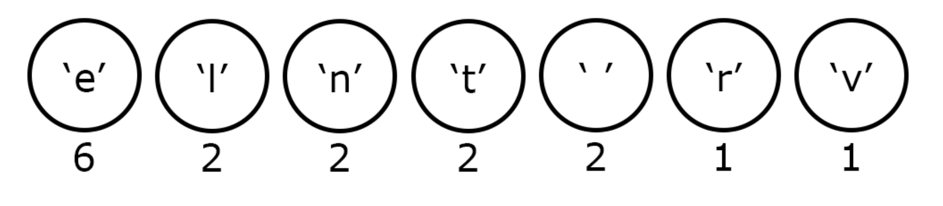
\includegraphics[width=100mm]{img/literatuurstudie/huffman-stap-1.png}}
	\caption{Een voorbeeld van hoe het resultaat na stap 1 (\ref{sec:primitieve-technieken-voorbeeld-huffman-encoding-1}) van \gls{huffman-coding} er voor de zin “lennert eet veel” kan uitzien. De volgorde van bomen met eenzelfde frequentie mogen van plaats gewisseld worden.}
	\label{fig:huffman-stap-1}
\end{figure}
\FloatBarrier

\subsubsection{Huffman encoding stap 2: bomen samenvoegen}
\label{sec:primitieve-technieken-voorbeeld-huffman-encoding-2}
Als tweede stap moeten alle bomen samengevoegd worden tot één boom waarbij voorrang gegeven wordt aan diegene met het kleinste totaal van frequenties. Indien er evenveel frequenties zijn, heeft diegene met de kleinste diepte voorrang.

Een voorbeeld van hoe het resultaat van deze stap er voor de zin “lennert eet veel” kan uitzien is te vinden op figuur \ref{fig:huffman-stap-2}.

\FloatBarrier
\begin{figure}[h!]
	\fbox{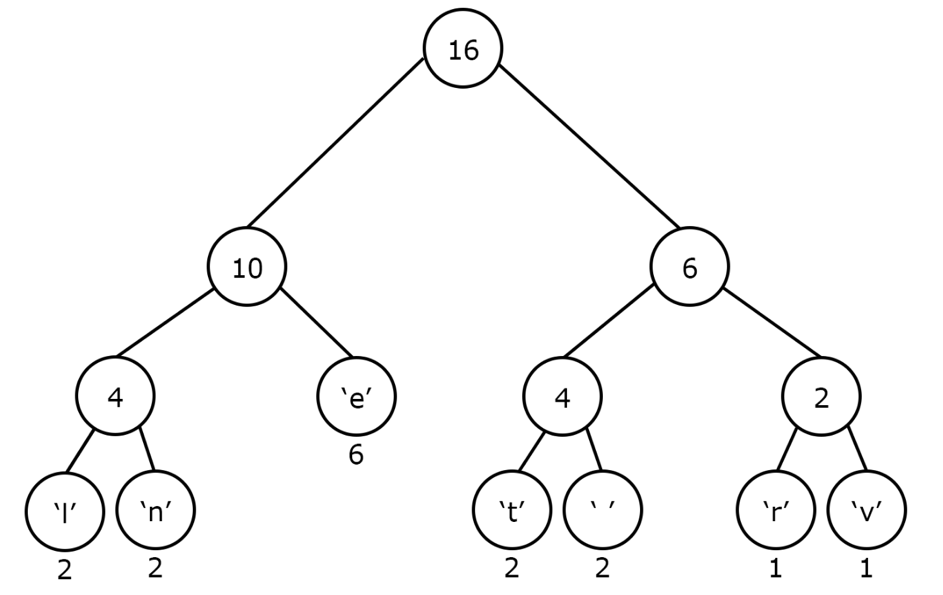
\includegraphics[width=100mm]{img/literatuurstudie/huffman-stap-2.png}}
	\caption{Een voorbeeld van hoe het resultaat na stap 2 (\ref{sec:primitieve-technieken-voorbeeld-huffman-encoding-2}) van \gls{huffman-coding} er voor de zin “lennert eet veel” kan uitzien. De knopen van een karakter met eenzelfde frequentie kunnen in sommige gevallen van plaats gewisseld worden.}
	\label{fig:huffman-stap-2}
\end{figure}
\FloatBarrier

\subsubsection{Huffman encoding stap 3: prefix tabel (optioneel)}
\label{sec:primitieve-technieken-voorbeeld-huffman-encoding-3}
Als derde, optionele, stap kan voor elk karakter de \gls{prefix-code} gemaakt worden en bijgehouden worden in een \gls{lookup-table}. Dit wordt gedaan door het pad naar het blad van het karakter bij te houden startend uit het hoofd waarbij een stap naar links als 0 genoteerd wordt en een stap naar rechts als 1.

Het is ook mogelijk deze berekening van het pad steeds opnieuw te doen en dus geen gebruik te maken vaan een \gls{lookup-table}.

De bekomen binaire boom van stap \ref{sec:primitieve-technieken-voorbeeld-huffman-encoding-2} levert onderstaande \gls{lookup-table} op.

\FloatBarrier
\begin{table}[h!]
	\begin{tabular}{|l|l|}
		\hline
		\textbf{karakter} & \textbf{prefix} \\ \hline
		'e'               & 01              \\ \hline
		'l'               & 000             \\ \hline
		'n'               & 001             \\ \hline
		't'               & 100             \\ \hline
		' '               & 101             \\ \hline
		'r'               & 110             \\ \hline
		'v'               & 111             \\ \hline  
	\end{tabular}
\end{table}
\FloatBarrier

\subsubsection{Huffman encoding stap 4: encoding}
\label{sec:primitieve-technieken-voorbeeld-huffman-encoding-4}
Als vierde en laatste stap kan nu eenvoudigweg elk karakter vervangen worden door zijn bijhorende \gls{prefix-code}. De zin “lennert eet veel” wordt door de bovenstaande \gls{lookup-table} voorgesteld als:
"000 01 001 001 01 110 100 101 01 01 100 101 111 01 01 000"

Het valt direct op dat deze reeks van \glspl{bit} (42 \glspl{bit}) veel kleiner is als in het \gls{ascii} voorbeeld (128 \glspl{bit}). Dit is de reden dat \gls{huffman-coding} tot op heden de grondlegger is voor veel \glspl{compressie-algoritme}. Hoewel \gls{huffman-coding} \gls{lossless} is en dus voornamelijk in andere \gls{lossless} \glspl{compressie-algoritme} gebruikt wordt, is \gls{huffman-coding} ook te vinden als onderdeel van tal van \gls{lossy} \glspl{compressie-algoritme}.


\subsubsection{Huffman decoding}
\label{sec:primitieve-technieken-voorbeeld-huffman-decoding}
De \gls{decoding} is visueel het eenvoudigst met behulp van de binaire boom door links en rechts te gaan afhankelijk van de bit. Bij het vinden van een blad is een karakter gevonden en kan recursief terug van het hoofd begonnen worden. Binnen het \gls{compressie-algoritme} zal een soort van \gls{lookup-table} gebruikt worden dat samen met het gecomprimeerd bestand dient opgeslagen te worden.

\subsubsection{Huffman coding Probleemstelling 1: binaire boom niet opgeslagen}
\label{sec:primitieve-technieken-voorbeeld-huffman-probleem-1}
In het voorgaande deel (\ref{sec:primitieve-technieken-voorbeeld-huffman-decoding}) is bewezen dat via de \gls{huffman-coding} reeks en de oorspronkelijke binaire boom het oorspronkelijk bericht volledig terug kan opgehaald worden (of via de \gls{lookup-table}). Er is echter enkel rekening gehouden met de \gls{huffman-coding} reeks voor het bepalen van de bestandsgrootte. Volgens die logica zou de originele binaire boom (of lookup table) dus niet opgeslagen worden en bijgevolg zou de originele tekst niet meer te reconstrueren zijn. Een soort \gls{lookup-table} zal dus ook moeten opgeslagen worden als \gls{meta-data}.


\subsubsection{Huffman coding Probleemstelling 2: gecomprimeerd bestand groter dan bron}
Zoals in probleemstelling \ref{sec:primitieve-technieken-voorbeeld-huffman-probleem-1} besproken is moet een soort \gls{lookup-table} bijgehouden worden als \gls{meta-data} voor het gecomprimeerd bestand. Dit veroorzaakt echter een volgend potentieel probleem .


Wanneer zowel de \gls{huffman-coding} reeks als de binaire zoekboom moeten opgeslagen worden bestaat de kans dat het gecomprimeerde bestand een grotere bestandsgrootte heeft dan het oorspronkelijk (door \gls{ascii} encoded) bestand. De mogelijkheid dat een gecomprimeerd bestand groter is dan een niet gecomprimeerd bestand is wederkerend bij \gls{datacompressie} en \gls{lossless} compressie in het bijzonder.


\subsubsection{Huffman coding Probleemstelling 3: overlappende prefix codes}
\label{sec:primitieve-technieken-voorbeeld-huffman-probleem-3}
\label{sec:primitieve-technieken-voorbeeld-huffman-probleem-2}
Door het gebruik van een binaire boom waarbij elk karakter voorgesteld wordt door een blad is het onmogelijk om een \gls{prefix-code} te bekomen die het begin is van een andere \gls{prefix-code}. In dit geval zou namelijk een knoop zijn aangeduid en geen blad (karakter).

Vooraleer er gebruik gemaakt werd van een binaire boom voor het bepalen van de \glspl{prefix-code} en het maken van de \gls{lookup-table} was dit echter wel een probleem. Zo konden \glspl{prefix-code} als 00, 001 en 00100 gelijktijdig voorkomen wat voor een gecomprimeerd bestand zorgt dat nooit met 100\% zekerheid gedecomprimeerd kan worden.

\section{Lossless vs lossy datacompressie}
\label{sec:ontstaan-datacompressie-lossless-lossy}
Zoals in hoofdstuk \ref{ch:termen} gedefinieerd slaat \gls{lossless} en \gls{lossy} op een categorie voor \glspl{compressie-algoritme}.
Bij \gls{lossless} \gls{datacompressie} is er geen verlies van 'kwaliteit' terwijl dit bij \gls{lossy} \gls{datacompressie} geen garantie is.

Het besproken \gls{huffman-coding} principe valt onder \gls{lossless} \gls{datacompressie}. Immers, de originele boodschap (en eender welke vorm van input) is bit per bit reconstrueerbaar door het \gls{compressie-algoritme}, er gaat dus geen data verloren. Een bit per bit reconstrueerbare clone is echter geen garantie voor \gls{lossless} \glspl{compressie-algoritme} aangezien \gls{meta-data} en andere zaken die geen impact hebben op “kwaliteit” wel verloren kunnen gaan.

Een typische \gls{use-case} voor \gls{lossless} \gls{datacompressie} zijn tekstdocumenten, de eindgebruiker wilt namelijk niet dat na het comprimeren letters verloren gaan in het document. 

Zoals reeds besproken in deel \ref{sec:ontstaan-datacompressie-primitieve-technieken-binnen-it} was de doorbraak van \gls{lossy} \gls{datacompressie} de opkomst van digitale afbeeldingen en muziek. Zo behoudt MP3 (\gls{lossy} \gls{codec} voor audio) bepaalde (combinaties van) audiofrequenties niet omdat die door het menselijke oor niet waarneembaar zijn. Maar ook waarneembare frequenties kunnen door de MP3 \gls{codec} verloren gaan voor het besparen van data. \gls{jpeg} is één van de oudste en bekendste vormen van \gls{lossy} \gls{compressie-algoritme} voor afbeeldingen. 

Zoals besproken in \citetitle{kaur2016} (\cite{kaur2016}) kunnen audiobestanden door het gebruik van \gls{lossy} \gls{datacompressie} tot 90\% kleiner worden in bestandsgrootte zonder een storende vermindering aan kwaliteit. Bij video kan een een nog grotere databesparing voorkomen, tot meer dan 99\% zonder dat daar veel visueel waarneembaar verschil mee gepaard gaat. Immers, opeenvolgende beelden lijken meestal erg op elkaar. Bij stilstaande afbeeldingen is het kwaliteitsverlies door \gls{lossy} \gls{datacompressie} vaak wel zeer zichtbaar wanneer 90\% of meer aan bestandsgrootte bespaard wordt.

De keuze voor \gls{lossless} of \gls{lossy} is \gls{use-case} gebonden. Bij het kiezen voor \gls{lossless} \gls{datacompressie} is een objectief onderzoek naar een goede balans tussen snelheid en databesparing voor de use case aangeraden. Bij \gls{lossy} \gls{datacompressie} zijn zowel objectieve als subjectieve onderzoeken mogelijk. In hoofdstuk \ref{ch:kwaliteit} wordt dieper ingegaan op de verschillende manieren om de prestatie van een \gls{compressie-algoritme} voor afbeeldingen te evalueren. In hoofdstuk \ref{ch:onderzoek} wordt een subjectief onderzoek gevoerd voor het bepalen van het geschikte \gls{afbeeldingsformaat} voor een bepaalde \gls{use-case}.

